% introduce experiment 4 
% problem setup 1
% estimand 4
% estimators 2
% variance + clt 2
% variance estimator + conservativeness + ci 1
% regression 1

\documentclass[aspectratio=169]{beamer}
\usetheme{default}
% \usecolortheme{default}
\setbeamertemplate{footline}[frame number]
\setbeamertemplate{navigation symbols}{}

% Fonts and encodings
\usepackage[utf8]{inputenc}
\usepackage[english]{babel}

% Math
\usepackage{amsmath, amsfonts, amssymb, mathtools, bm}
\usepackage{bbm}

% Graphics & hyperlinks
\usepackage{graphicx}
\usepackage{tikz}
\usetikzlibrary{positioning,chains,fit,shapes,calc}
\usepackage{hyperref}
\hypersetup{colorlinks=true, linkcolor=blue, citecolor=blue, urlcolor=blue}

% Bibliography
\usepackage[authoryear]{natbib}
\bibliographystyle{apalike}

% Colors
\definecolor{myblue}{RGB}{80,80,160}
\definecolor{mygreen}{RGB}{80,160,80}

% Define math operators
\DeclareMathOperator*{\argmax}{argmax}
\DeclareMathOperator*{\argmin}{argmin}
\DeclareMathOperator{\tr}{tr}
\DeclareMathOperator{\vect}{vec}
\DeclareMathOperator{\Rank}{Rank}

% Define shortcut
\newcommand{\E}{\mathbb{E}}
\newcommand{\B}{B}
\newcommand{\Var}{\mathrm{Var}}
\newcommand{\Cov}{\mathrm{Cov}}
\newcommand{\bbm}[1]{\mathbbm{#1}}
\newcommand{\bb}[1]{\mathbb{#1}}
\newcommand{\floor}[1]{\lfloor #1 \rfloor}
\newcommand{\sq}[1]{\textquoteleft #1 \textquoteright}
\newcommand{\dq}[1]{\textquotedblleft #1 \textquotedblright}
\newcommand{\red}{\color{red}}
\newcommand{\norm}[1]{\left\lVert#1\right\rVert}
\def\T{{\textsc{t}}}

\newcommand{\pr}{\textup{pr}}
\newcommand{\cov}{\textup{cov}}
\newcommand{\var}{\textup{var}}
\newcommand{\avar}{\textup{avar}}
\newcommand{\acov}{\textup{acov}}
\newcommand{\kprime}{k^{\prime}}
\newcommand{\adj}{\textup{adj}}

\newcommand{\bOneZ}{\boldsymbol{1}_{m}}
\newcommand{\bZeroZ}{\boldsymbol{0}_{m}}
\newcommand{\bOneA}{\boldsymbol{1}_{n}}
\newcommand{\bZeroA}{\boldsymbol{0}_{n}}
\newcommand{\Yt}[1]{Y_{#1}(\boldsymbol{1}_{m})}
\newcommand{\Yc}[1]{Y_{#1}(\boldsymbol{0}_{m})}

\newcommand{\bY}{\boldsymbol{Y}}
\newcommand{\bz}{\boldsymbol{z}}
\newcommand{\bZ}{\boldsymbol{Z}}
\newcommand{\ba}{\boldsymbol{a}}
\newcommand{\bA}{\boldsymbol{A}}
\newcommand{\bW}{\boldsymbol{W}}
\newcommand{\bV}{\boldsymbol{V}}
\newcommand{\bX}{\boldsymbol{X}}
\newcommand{\bpi}{\boldsymbol{\pi}}
\newcommand{\Davg}{D_{\textup{avg}}}
\newcommand{\bOmega}{\boldsymbol{\Omega}}

\newcommand{\cN}{\mathcal{N}}
\newcommand{\cF}{\mathscr{F}}
\newcommand{\cT}{\mathcal{T}}
\newcommand{\cS}{\mathcal{S}}

\newcommand{\tA}{\tilde{A}}
\newcommand{\tS}{\tilde{S}}
\newcommand{\tH}{\tilde{H}}


\newcommand{\allt}{\left(\prod_{k\in \mathcal{G}_{+i}} Z_k\right)}
\newcommand{\alltj}{\left(\prod_{k\in \mathcal{G}_{+j}} Z_k\right)}
\newcommand{\allc}{\left\{\prod_{k\in \mathcal{G}_{+i}} (1-Z_k)\right\}}
\newcommand{\allcj}{\left\{\prod_{k\in \mathcal{G}_{+j}} (1-Z_k)\right\}}

\newcommand{\plim}{\textup{plim}}

\newcommand{\bG}{\boldsymbol{G}}
\newcommand{\bGamma}{\boldsymbol{\Gamma}}
\newcommand{\G}{G}
\newcommand{\cG}{\mathcal{G}}
\newcommand{\cGijcap}{\cG_{+i} \cap \cG_{+j}}
\newcommand{\cGijcup}{\cG_{+i} \cup \cG_{+j}}

\newcommand{\Smax}{{\max_{1\leq i\leq n}\G_{+i}}}
\newcommand{\Dmax}{{\max_{1\leq k\leq m}\G_{k+}}}
\newcommand{\Smaxsupp}{{\bar{D}_\textup{O}}}
\newcommand{\Dmaxsupp}{{\bar{D}_\textup{I}}}

\newcommand{\sumi}{\sum_{i=1}^n}
\newcommand{\sumj}{\sum_{j=1}^n}
\newcommand{\sumk}{\sum_{k=1}^m}
\newcommand{\sumij}{\sum_{i=1}^{n} \sum_{j=1}^{n}}
\newcommand{\sumjneqi}{\sum_{j\neq i}}
\newcommand{\sumu}{\sum_{u=1}^n}
\newcommand{\sumv}{\sum_{v=1}^n}
\newcommand{\maxi}{\max_{1\leq i\leq n}}

\newcommand{\de}{\textsc{de}}
\newcommand{\bie}{\textsc{bie}}
\newcommand{\wie}{\textsc{wie}}
\newcommand{\horthom}{\textup{ht}}
\newcommand{\haj}{\textup{haj}}
\newcommand{\diag}{\textup{diag}}

\newcommand{\indicator}{\mathbbm{1}}
\newcommand{\bbI}{\mathbbm{I}}
\newcommand{\ashprime}{a^{\prime},s^{\prime},h^{\prime}}

% propensity scoressssss
\newcommand{\pscore}[1]{\pi_{#1}}

\newcommand{\sz}[1]{{\textcolor{olive}{(Sizhu: #1)}}}

\makeatletter
\newcommand{\ostar}{\mathbin{\mathpalette\make@circled\star}}
\newcommand{\make@circled}[2]{%
  \ooalign{$\m@th#1\smallbigcirc{#1}$\cr\hidewidth$\m@th#1#2$\hidewidth\cr}%
}
\newcommand{\smallbigcirc}[1]{%
  \vcenter{\hbox{\scalebox{0.77778}{$\m@th#1\bigcirc$}}}%
}
\makeatother



% Title
% \title[Spillovers in Randomized Saturation Designs]{Estimating within-cluster and between-cluster spillover effects in randomized saturation designs}
% \author[S. Lu, L. Shi, P. Ding]{Sizhu Lu\and Lei Shi\and Peng Ding}
% \institute[UC Berkeley]{University of California, Berkeley}
% \date{\today}

% Title
\title[]{Estimating within-cluster and between-cluster spillover effects in randomized saturation designs}
\author[S. Lu, L. Shi, P. Ding]{Sizhu Lu$^{\ast}$\and Lei Shi$^{\ast}$\and Peng Ding}
\institute[UC Berkeley]{
  University of California, Berkeley \\[0.4em]
  \normalsize Workshop on causal network analysis, Emory University
}
\date{August 14, 2025}


\AtBeginSection[]
{
  \begin{frame}
    \frametitle{Outline}
    \tableofcontents[currentsection]
  \end{frame}
}

\begin{document}

% Title page
\begin{frame}
  \titlepage
\end{frame}


\section{Introduction}
\begin{frame}{Motivating example: large-scale cash transfer experiment in rural Kenya}
\begin{columns}[T] % Align columns at top
  \begin{column}{0.45\textwidth}
    \begin{itemize}
      \item Two-stage \emph{randomized saturation} design \citep{egger2022general}:
        \begin{itemize}
          \item \textbf{Stage 1:} Sublocations randomized to high and low saturation.
          \item \textbf{Stage 2:} Villages randomized to treatment at the assigned saturation rate.
        \end{itemize}
      \item Geography (markets, labor, mobility) induces interference \emph{within} and \emph{between} sublocations.
    \end{itemize}
  \end{column}
  \begin{column}{0.55\textwidth}
    \centering
    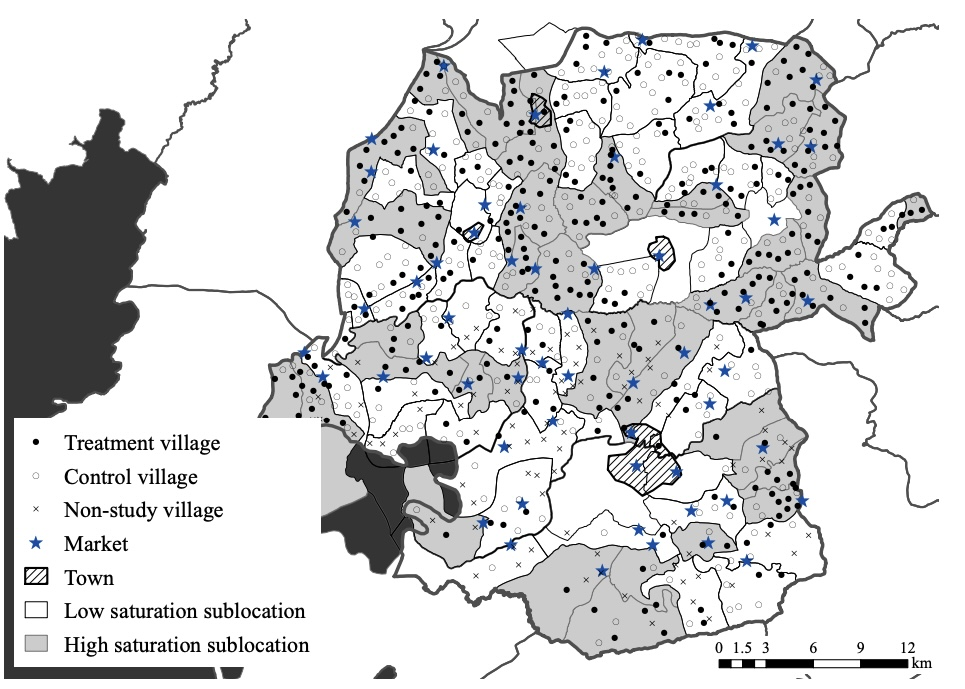
\includegraphics[width=\linewidth]{spatial.jpg}
  \end{column}
\end{columns}
\end{frame}

\begin{frame}{Spatial exposure to treatment}
  \centering
  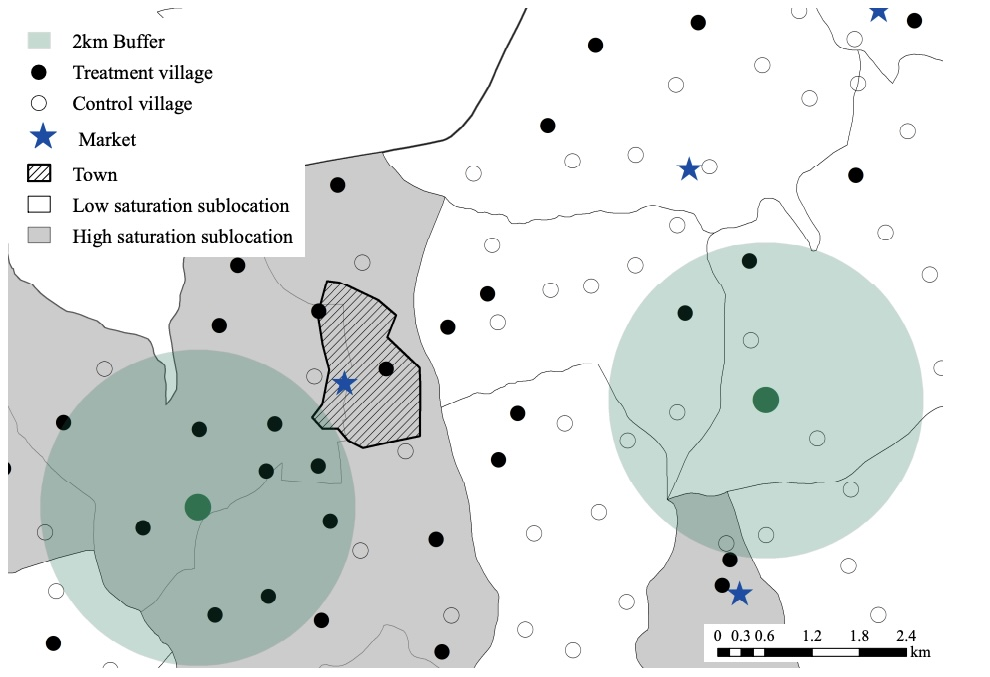
\includegraphics[width=0.5\textwidth]{spatial-political.jpg}
  \begin{itemize}
    \item Evidence of meaningful \textbf{spillovers} on non-recipient households and local markets.
    \item Positive effects on local enterprise activity and consumption reported.
  \end{itemize}
\end{frame}

% \begin{frame}{More applications}
% \begin{itemize}
%   \item \cite{hudgens2008toward}: Motivated by a cholera vaccine trial in Bangladesh (Ali et al., 2005). 
%     \begin{itemize}
%       \item Stage 1: Communities randomized to high and low vaccination coverage.
%       \item Stage 2: Individuals within each community randomized to vaccination at the assigned coverage rate.
%       \item Infectious disease transmission can occur via travel, markets, or shared water sources across community boundaries.
%     \end{itemize}
%     \pause
%   \item \cite{miguel2004worms}: Kenya school deworming RCT.
%     \begin{itemize}
%       \item Phased-in randomization at the school level over several years.
%       \item School catchment areas overlap through shared water sources and sibling attendance patterns, making between-school interference likely.
%     \end{itemize}
% \end{itemize}
% \end{frame}

\begin{frame}{Motivation}
\begin{itemize}
    \item Widely-used design: deworming on health \citep{miguel2004worms}, vaccination on health \citep{ali2005herd}, labor market policies on displacement \citep{crepon2013labor}, school governance on learning \citep{pradhan2014improving}, microcredit on business outcomes \citep{banerjee2015miracle}, education on fertility \citep{duflo2015education}, cash transfers on school attendance \citep{barrera2019long}.
    \pause
    \item Common assumption in prior work: spillovers \textbf{only} occur within clusters, no interference between clusters.
    \pause
    \item Not reasonable in many cases:
    \begin{itemize}
      \item Real-world clusters are rarely isolated.
      \item Networks, mobility, markets, or environmental channels can connect units across cluster boundaries.
      \item Ignoring between-cluster interference can bias effect estimates and mislead policy conclusions.
    \end{itemize} 
\end{itemize}
\end{frame}

\begin{frame}{Our contribution and roadmap}
\begin{itemize}
    \item Formalize analysis in randomized saturation designs, allowing for \emph{both} within- and between-cluster spillovers.
    \pause
    \item \textbf{Estimands}: Direct effect, within-cluster indirect effect, and between-cluster indirect effect.
    \pause
    \item \textbf{Estimators}: Design-based Horvitz--Thompson and H\'{a}jek estimators by inverse probability weighting.
    \pause
    \item \textbf{Inference}: Closed-form asymptotic variance, conservative variance estimators, CLTs, and Wald CIs. 
\end{itemize}  
\end{frame}


\begin{frame}{Notation and exposure mapping}
\begin{itemize}
% \item Two-stage design:
% \begin{itemize}
%       \item Stage 1: Randomly assign clusters (sublocations) to high and low saturation.
%       \item Stage 2: Within each sublocation, randomly assign villages to treatment at the assigned saturation rate.
% \end{itemize}
% \pause
\item $i$: unit/village index.
\item $A_i\in\{0,1\}$: treatment indicator.
\item $Y_i(\ba)$ for $\ba = (a_1,\ldots,a_n)^{\T}$: $2^n$ potential outcomes.
\pause
\item Exposure mapping $(A_i, S_i, H_i)$: reduces the high-dimensional dependence to a low-dimensional summary, where
\pause
\begin{itemize}
    \item $S_i$: within-cluster summary, e.g., whether $>1/2$ villages are getting treated within the same sublocation as $i$,
    \pause
    \item $H_i$: between-cluster summary, e.g., whether $>1/2$ villages are treated among those geographically close to $i$ but located in different sublocations.
\end{itemize}
\pause
\item Potential outcome reduces to $Y_i(a,s,h)$.
\pause
\item Finite population regime: fixed potential outcomes, randomness from treatment.
\end{itemize}
\end{frame}


% Causal parameters: direct effect
\section{Causal estimands}

\begin{frame}{Controlled direct and indirect effects}
\begin{itemize}
    \item The controlled direct effect of treatment $A_{i}$ on the outcome, while holding the exposure variables $(S_{i},H_{i})$ fixed at values $(s,h)$:
    {\small 
    \[
    \de(s,h) = n^{-1}\sumi Y_{i}(1,s,h) - n^{-1}\sumi Y_{i}(0,s,h).
    \]
    }
    \pause
    \item The within-cluster controlled indirect effect of $S_{i}$ on the outcome, holding $H_{i}$ fixed at $h$:
    {\small 
    \[
    \wie(s,s^{\prime},h) = n^{-1}\sumi Y_{i}(0,s,h) - n^{-1}\sumi Y_{i}(0,s^{\prime},h).
    \]
    }
    \pause
    \item The between-cluster controlled indirect effect of $H_{i}$ on the outcome, holding $S_{i}$ fixed at $s$:
    {\small
    \[
    \bie(s,h,h^{\prime}) = n^{-1}\sumi Y_{i}(0,s,h) - n^{-1}\sumi Y_{i}(0,s,h^{\prime}).
    \]
    }
\end{itemize}
\end{frame}

\begin{frame}{Marginal direct and indirect effects}
\begin{itemize}
    \item The marginal direct effect of treatment $A_{i}$, marginalizing over the distribution of treatments for all other villages:
    \begin{small}
    \[
    \de = n^{-1}\sumi \underbrace{E_{\bA_{(-i)}}\left\{Y_{i}(1,S_{i},H_{i})\right\}}_{\textup{distribution of }\bA_{(-i)}} - n^{-1}\sumi E_{\bA_{(-i)}}\left\{Y_{i}(0,S_{i},H_{i})\right\}.
    \]
    \end{small}
    \pause
    \item The within-cluster marginal indirect effect:
    \begin{small}
    \[
    \wie(s,s^{\prime}) = n^{-1}\sumi \underbrace{E_{\bA_{(-i)}\mid S_{i} = s}\left\{Y_{i}(0,s,H_{i})\right\}}_{\textup{conditional distribution }\bA_{(-i)}\textup{ given }S_{i}=s} - n^{-1}\sumi E_{\bA_{(-i)}\mid S_{i} = s^{\prime}}\left\{Y_{i}(0,s^{\prime},H_{i})\right\}.
    \]
    \end{small}
    \pause
    \item The between-cluster marginal indirect effect:
    \begin{small}
    \[
    \bie(h,h^{\prime}) = n^{-1}\sumi E_{\bA_{(-i)}\mid H_{i} = h}\left\{Y_{i}(0,S_{i},h)\right\} - n^{-1}\sumi E_{\bA_{(-i)}\mid H_{i} = h^{\prime}}\left\{Y_{i}(0,S_{i},h^{\prime})\right\}.
    \] 
    \end{small}
\end{itemize}
\end{frame}


\begin{frame}
\frametitle{Policy-specific direct and indirect effects}
\begin{itemize}
    \item For a given treatment policy $\psi$, define the policy-specific direct and indirect effects:
    \begin{small}
    \begin{align*}
    \de_\psi &= n^{-1}\sumi E_\psi\{Y_i(1,S_i,H_i)\} - n^{-1}\sumi E_\psi\{Y_i(0,S_i,H_i)\}, \\
    \wie_\psi &= n^{-1}\sumi E_\psi\{Y_i(0,1,H_i)\} - n^{-1}\sumi E_\psi\{Y_i(0,0,H_i)\}, \\
    \bie_\psi &= n^{-1}\sumi E_\psi\{Y_i(0,S_i,1)\} - n^{-1}\sumi E_\psi\{Y_i(0,S_i,0)\},
    \end{align*}
    \end{small}
    \begin{itemize}
        \item subscript $\psi$: expectation under distribution of $(S_{i}, H_{i})$ conditional on $A_{i} = a$ induced by policy $\psi$ for $a=0,1$.
    \end{itemize}
    \item Comparison between different policies $\psi_1$ vs $\psi_2$, e.g., $\de_{\psi_1} - \de_{\psi_2}$.
\end{itemize}
\end{frame}

\section{Estimation}
\begin{frame}
\frametitle{Estimators for controlled effects}
\begin{itemize}
    \item Solution: estimate each average potential outcome $n^{-1}\sumi Y_i(a,s,h)$:
    \pause 
    \begin{itemize}
        \item Define $\bbI_{i}(a,s,h)=\indicator\{A_{i}=a,S_{i}=s,H_{i}=h\}$ and $\pscore{i}(a,s,h)=\pr(A_{i}=a, S_{i}=s, H_{i}=h)$.
        \pause 
        
        \item Horvitz--Thompson estimator: 
        $$\hat{Y}^{\horthom}(a,s,h) = n^{-1}\sumi\frac{\bbI_{i}(a,s,h)}{\pscore{i}(a,s,h)}Y_i.$$
        \pause 
        
        \item H\'{a}jek estimator:
        $$\hat{Y}^{\haj}(a,s,h) = n^{-1}\sumi\frac{\bbI_{i}(a,s,h)}{\pscore{i}(a,s,h)}Y_i \Big / n^{-1}\sumi\frac{\bbI_{i}(a,s,h)}{\pscore{i}(a,s,h)}.$$
        \pause 
        
        \item Propensity scores can be \textbf{simulated} from the design and the network structure. 
        \pause 
    \end{itemize}
    \item Controlled effect can be estimated by differences between these average estimators.
\end{itemize}
\end{frame}

% Policy-specific reweighting
\begin{frame}{Estimators for policy-specific effects}
\begin{itemize}
    \pause 
    \item Solution: need to reweight to target a different policy. 
    \pause 
    
    \item Let $\Gamma = \{\gamma_i(a,s,h)\}$ be a set of prespecified unit weights to target different effects. 
    \pause
    
    \item Horvitz--Thompson estimators:
    \begin{small}
    \begin{eqnarray*}
        \hat{Y}^{\horthom}(a,s,h;\Gamma) &=& n^{-1}\sumi\frac{ \bbI_{i}(a,s,h)\gamma_i(a,s,h)}{ \pscore{i}(a,s,h)}Y_{i}. 
    \end{eqnarray*}
    \end{small}
    \pause
    
    \item H\'{a}jek-type estimator
    \begin{small}
    \begin{equation*}
    \hat{Y}^{\haj}(a,s,h) = n^{-1}\sumi \gamma_i(a,s,h)\cdot n^{-1}\sumi\frac{ \bbI_{i}(a,s,h) \gamma_i(a,s,h)}{ \pscore{i}(a,s,h)}Y_{i} \Big / n^{-1}\sumi\frac{ \bbI_{i}(a,s,h) \gamma_i(a,s,h)}{ \pscore{i}(a,s,h)}. 
    \end{equation*}
    \end{small} 
\end{itemize}
  


\end{frame}

\begin{frame}{Choice of weights}
\begin{itemize}
\pause 
    \item Choose weights to target policy \(\psi\) for different effects: 
    {\small 
  \[
    \gamma^{\de}_{i,\psi}(a,s,h)=\pi_{i,\psi}(\cdot,s,h),\quad
    \gamma^{\wie}_{i,\psi}(a,s,h)=\pi_{i,\psi}(\cdot,\cdot,h),\quad
    \gamma^{\bie}_{i,\psi}(a,s,h)=\pi_{i,\psi}(\cdot,s,\cdot).
  \]}\pause 
   \item All of the above weights can be simulated based on the design.
\pause   

  \item Can be used to construct estimators for the policy-specific effects: for \(*\in\{\horthom,\haj\}\),
  {\small 
  \begin{eqnarray*}
    \hat{\de}_{\psi}^{*} &=& \sum_{s,h=0,1} \{\hat{Y}^{*}(1,s,h;\Gamma_{\psi}^{\de})  - \hat{Y}^{*}(0,s,h;\Gamma_{\psi}^{\de})\}, \\
    \hat{\wie}_{\psi}^{*} &=& \sum_{h=0,1} \{\hat{Y}^{*}(0,1,h;\Gamma_{\psi}^{\wie}) - \hat{Y}^{*}(0,0,h;\Gamma_{\psi}^{\wie})\}, \\
    \hat{\bie}_{\psi}^{*} &=& \sum_{s=0,1} \{\hat{Y}^{*}(0,s,1;\Gamma_{\psi}^{\bie}) - \hat{Y}^{*}(0,s,0;\Gamma_{\psi}^{\bie})\}.
\end{eqnarray*}
} 
\pause 

    \item Marginal direct/indirect effects are a special case with the implemented policy. 
\end{itemize}
    
\end{frame}


\section{Theoretical properties}

\begin{frame}
\frametitle{Asymptotic variance: Horvitz--Thompson}
\begin{itemize}
    \item For the Horvitz-Thompson estimator:
    \pause 
    {\small 
\begin{align*}
\var\{\hat{Y}^{\horthom}(a,s,h;\Gamma)\} 
&= \underbrace{n^{-2}\sumi \frac{1-\pscore{i}(a,s,h)}{\pscore{i}(a,s,h)}\{\gamma_i(a,s,h)Y_i(a,s,h)\}^2}_{\text{contribution from the variation of unit $i$}} \\
&\quad + n^{-2}\sumi\sum_{j\neq i}\frac{\pscore{ij}(a,s,h;a,s,h) - \pscore{i}(a,s,h)\pscore{j}(a,s,h)}{\pscore{i}(a,s,h)\pscore{j}(a,s,h)} \\
&\qquad \underbrace{\phantom{hello}\times \gamma_i(a,s,h)\gamma_j(a,s,h)Y_i(a,s,h)Y_j(a,s,h).\phantom{hello}}_{\text{contribution from the covariance between units due to interference}}
\end{align*}
} 
\pause 

\item  Can be written compactly as:
$$\var\{\hat{Y}^{\horthom}(a,s,h;\Gamma)\} = n^{-2}\bY(a,s,h)^T\bGamma(a,s,h)\bOmega(a,s,h)\bGamma(a,s,h)\bY(a,s,h).$$
\end{itemize}

\end{frame}

\begin{frame}
\frametitle{Asymptotic variance: H\'{a}jek estimator}

\begin{itemize}
    \item For the H\'{a}jek estimator:

    \begin{itemize}
    \pause 
        \item in the same form of the Horvitz-Thompson variance, only with $\bY(a,s,h)$ replaced by \textbf{the centered potential outcomes} $\tilde\bY(a,s,h)$. 
    \pause 
        \item The centered potential outcomes are:
        $$\tilde{Y}_i(a,s,h) = Y_i(a,s,h) - \frac{n^{-1}\sumi \gamma_i(a,s,h)Y_i(a,s,h)}{n^{-1}\sumi\gamma_i(a,s,h)}$$
    \pause 
        \item Compactly: $n^{-2}\tilde{\bY}(a,s,h)^T\bGamma(a,s,h)\bOmega(a,s,h)\bGamma(a,s,h)\tilde{\bY}(a,s,h)$. 
    \end{itemize}
    \pause 

   \item Can give conditions for the consistency of the estimators.
   \pause 

   \item This centering properties explain why empirically, the H\'{a}jek estimator is usually more stable

\end{itemize}

\end{frame}

\begin{frame}
\frametitle{Covariance structure}
\begin{itemize}
    \item Horvitz--Thompson covariance
    for $(a,s,h) \neq (a',s',h')$:
    \pause 
    \begin{align*}
    &\cov\{\hat{Y}^{\horthom}(a,s,h;\Gamma), \hat{Y}^{\horthom}(a',s',h';\Gamma)\} \\
    &= \underbrace{-n^{-2}\sumi \gamma_i(a,s,h)\gamma_i(a',s',h')Y_i(a,s,h)Y_i(a',s',h')}_{\text{Covariance of different potential outcomes for the same unit $i$}} \\
    &\quad + n^{-2}\sumi\sum_{j\neq i}\frac{\pscore{ij}(a,s,h;a',s',h') - \pscore{i}(a,s,h)\pscore{j}(a',s',h')}{\pscore{i}(a,s,h)\pscore{j}(a',s',h')} \\
    &\qquad \underbrace{\phantom{hello}\times \gamma_i(a,s,h)\gamma_j(a',s',h')Y_i(a,s,h)Y_j(a',s',h')\phantom{hello}}_{\text{Covariance of different potential outcomes between units}}
    \end{align*}

    \pause 
    \item {H\'{a}jek covariance:} Same form but with centered potential outcomes $\tilde{Y}_i(a,s,h)$ and $\tilde{Y}_j(a',s',h')$
\end{itemize}

\end{frame}

\begin{frame}{CLT and confidence intervals}
    \begin{itemize}
    \pause 
        \item One ongoing technical work is developing central limit theorems and confidence intervals for the proposed estimators;
    \pause 

        \item Central limit theorem: potentially use Stein's method to capture correlation due to network interference and characterize asymptotic distributions;
    \pause 

        \item Confidence interval: relies on constructing valid variance estimators. 
    \end{itemize}
\end{frame}

\section{Additional results}

% Regression-based analysis
\begin{frame}{Regression-based analysis}
\begin{itemize}
    \item What if we analyze the experiments in a factorial regression flavor? 
    \pause 
    \item \textbf{Partially saturated regression:}
  \[
    Y_i \sim 1 + A_i + \tilde S_i + \tilde H_i + A_i\tilde S_i + A_i \tilde H_i,
  \]
  where \(\tilde S_i\) and \(\tilde H_i\) are centered indicators using population means. Then:
  \begin{itemize}
  \pause 
    \item Coefficient on \(A_i\) targets the marginal direct effect $\de$.
  \pause 
    \item Centering yields ``overlap'' versions of indirect effects; exact $\wie$ and $\bie$ recovery requires weighting.
  \end{itemize}
  \pause 
  \item See \citet{zhao2022regression, aronow2017estimating}.
\end{itemize}
  
\end{frame}

\begin{frame}{Ongoing work}
\begin{itemize}
    \item Covariate adjustment: 
    \begin{itemize}
    \pause 
        \item How to use pre-treatment covariates to enhance the efficiency of the estimators?
        \begin{itemize}
            \item Demographic features, characteristics of the graph, etc.
        \end{itemize}
    \pause 
        \item Many classic discussions on \textit{model-assisted} regression adjustment using pretreatment covariates, \textbf{without assuming the true outcome model}.
    \pause 
        \item Adapting the framework to the current setting is a future step to enhance the analysis.

    \end{itemize}
    \pause 

    \item Experimental validation:
    \begin{itemize}
    \pause
        \item The Cash Transfer experiment has a publicly available dataset.
    \pause 
        \item Working on experimental validation with this study.
    \end{itemize}
\end{itemize}
    
\end{frame}


% % Practical notes
% \begin{frame}{Practical notes}
%   \begin{itemize}
%     \item Between-cluster neighbors for isolated units:
%     \begin{itemize}
%       \item Define a nearest non-cluster neighbor set to ensure \(H_i\) is defined; or
%       \item Set \(H_i=0\) for isolated units (may violate overlap and affect variance ID \citep{aronow2017estimating}).
%     \end{itemize}
%     \item Inference relies on known design probabilities; estimate or simulate when closed forms are complex.
%   \end{itemize}
% \end{frame}

% References
\begin{frame}[allowframebreaks]{References}
  \footnotesize
  \bibliography{ref}
\end{frame}

\end{document}